\chapter{Einleitung}
\label{cha:Einleitung}

\section{Was ist Linux?}

Unter dem Begriff Linux versteht man allgemein einen Ueberbegriff fuer freie Betriebssysteme, welche auf dem Linux Kernel basieren. Der Linux Kernel wurde erstmals im frühjahr 1992 unter der GNU GPL Lizenz fuer Intels x86 Architektur veroeffentlicht.

Ein konkretes Linux Betriebssystem bezeichnet man als Linux Distribution. Eine Distribution besteht aus einem Linux Kernel, GNU Tools und Libraries, zusaetzlicher Software und manchmal auch einem Window System, einem Windows Manager und einem Desktop Environment. Beispiele fuer solche Linux Distributionen sind Debian, Ubuntu, Arch Linux, openSUSE, Fedora und Linux on z.

\section{Linux Kernel Architekturen}

Der Linux Kernel ist von monolithischer aber auch modularer Natur. Dies bedeutet, dass Funktionalitaeten, welche der Kernel zwingend braucht, direkt eingebaut sind - Funktionalitaeten welche aber nur bei ganz bestimmten Hardwarekomponenten gebraucht werden, koennen ueber sogenannte Kernel Module nachgeladen werden.
Der Linux Kernel uebernimmt Aufgaben wie beispielsweise die Speicher- und Prozessverwaltung, Interprozesskommunikation, Geraeteverwaltung und Dateisystem.
Nachfolgende Grafik zeigt eine Uebersicht wichtiger Aufgaben des Linux Kernels im Zusammenspiel mit Hardware und den Userspace Anwendungen der Distribution:

\begin{figure}[h!]
\centering
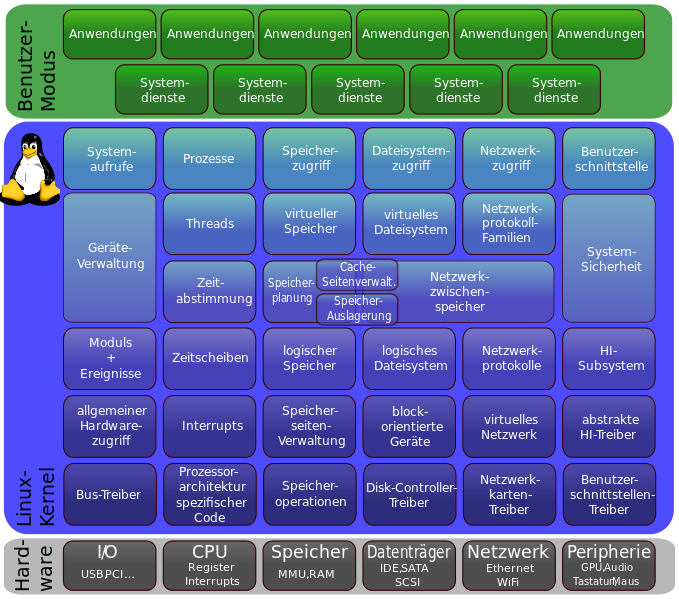
\includegraphics[width=.80\textwidth]{einleitung-kernel-struktur}
\caption{Linux Kernel Struktur\cite{KernelStruktur}.}
\label{fig:KernelStruktur}
\end{figure}

\newpage

Dieser modular-monolithischer Ansatz des Linux Kernels traegt nicht zuletzt zu seiner grossen Verbreitung auf unterschiedlichsten Architekturen und Plattformen bei.

Wikipedia fuehrt eine Liste der Computer Architekturen, welche Linux unterstuetzt.
Inzwischen sind dort ueber 100 Architekturen zu finden. Diese breite Abdeckung von Architekturen macht es moeglich, dass Linux in beinahe alle Bereiche von Betriebssystem Umgebungen Einzug gefunden hat. Diese reicht von exotischen Umgebungen, wie Navigations- und Haushaltsgeraeten, Digitalkameras, ueber Desktop- und Laptop Computern und Mobiltelefonen mit Android, bis hin zu Supercomputern und High Performance Computing Clusters mit Rocks Cluster Distribution.

So hat Linux auch seine Daseinsberechtigung auf dem Mainframe gefunden mit Linux on z, welches auf IBMs z Systems und IBMs LinuxONE laeuft.
